% Provenance (never printed): see sources/outline_sources.md (Year 1: internal
% structure of the Earth from seismology; reference model; density, gravity and
% pressure inside the Earth; mantle mineralogy; lithosphere and asthenosphere).
% Curves from figdata/bachelor-1/prem_profiles.py (shared dataset data:prem) and
% figdata/bachelor-1/refraction.py (generic two-layer crust); exercise and problem
% values in the Book 3 scratch calculator calc/ch09.py.
\chapter{成层地球}\label{ch:b1:layered-earth}

1909 年 10 月 8 日，一场地震震动了萨格勒布东南方的库帕山谷。
% ledger: skoko:mohorovicic
当地天文台主持人安德里亚·莫霍洛维奇收集了欧洲各地记录的地震图，
并发现一个奇特现象：在距震中数百千米以内，
首先到达的震动以一种方式传来；更远处则由另一类先到的震动接替，
仿佛部分能量在地下深处找到了一条更快的路径。
他用地下约五十千米处的一个界面解释了这一现象，该界面以下波速更快，
即\omterm{def:b1:layered-earth:layers}{地壳}的底界。
一个世纪以来，数以百万计的此类记录，
把这一最初的界面发展成了整个地球的参考模型，逐层给出速度、密度、
重力以及直到地心的压强。本章将说明如何由走时确定界面，
参考模型说明了什么，如何仅由地震波速画出密度剖面，
并用地球的质量与转动惯量加以检验，
\omterm{def:b1:layered-earth:layers}{地幔}在各深度由哪些\omterm{def:b1:rock-forming-minerals:mineral}{矿物}组成，
地核由什么构成，以及行星的刚性外壳在何处
结束。

\begin{recall}
P 波是压缩波，S 波是剪切波；S 波不能穿过液体，
地核的 P 波与 S 波影区给出了液态\omterm{def:b1:layered-earth:layers}{外核}的半径（第 2 册，十一年级）。
波在界面处按斯涅耳定律发生折射，
即 $\sin i_1/v_1 = \sin i_2/v_2$（物理）。在静止流体中，
压强随深度增大，满足 $\mathrm dP = \rho g\,\mathrm dz$，
（物理，本科一年级）。\omterm{def:b1:layered-earth:layers}{地壳}、\omterm{def:b1:layered-earth:layers}{地幔}和地核在
第 1 册（六年级）中已经介绍过。
\end{recall}

\section{成层地球中的地震波}

地震波的速度取决于岩石的弹性模量与密度。
物理教材由连续介质弹性理论推导了这些结果，
此处直接取作已知。

\begin{proposition}[地震波速]\label{prop:b1:layered-earth:speeds}
设各向同性弹性固体的密度为 $\rho$，体变模量为 $K$，剪切模量为 $\mu$，
则 P 波与 S 波的速度分别为
\[
  v_P = \sqrt{\frac{K + \tfrac43\mu}{\rho}}, \qquad v_S = \sqrt{\frac{\mu}{\rho}}.
\]
在液体中 $\mu = 0$，$v_S = 0$，S 波不能传播。
\end{proposition}
\admitted

由于 $K$ 与 $\mu$ 均为正，恒有 $v_P > v_S$：
在 PREM 的\omterm{def:b1:layered-earth:layers}{地壳}与\omterm{def:b1:layered-earth:layers}{地幔}中，$v_P$ 约为 $1.8$ 至 $1.9$ 倍的 $v_S$，P 波先到达。
两种速度一般随深度增大，因为压强使岩石变硬的程度超过使其压缩的程度，
射线因而向地表弯回；在少数深度处，
速度发生跳变。

\begin{definition}[地震波速不连续面、莫霍面、核幔边界与内核边界]
\label{def:b1:layered-earth:discontinuity}
称地球内部的一个面为\emph{地震波速不连续面}\index{地震波速不连续面}，
若沿该面地震波速、密度或二者同时发生突变，
且突变所跨越的厚度远小于地震波的波长。
\emph{莫霍洛维奇不连续面}\index{莫霍洛维奇不连续面}（或
\emph{莫霍面}\index{莫霍面}）是\omterm{def:b1:layered-earth:layers}{地壳}的底界，在此 $v_P$ 跃变至
约 \qty{8}{km.s^{-1}}。\emph{核幔边界}\index{核幔边界}
是固态硅酸盐\omterm{def:b1:layered-earth:layers}{地幔}与液态\omterm{def:b1:layered-earth:layers}{外核}之间的面；
\emph{内核边界}\index{内核边界}是液态\omterm{def:b1:layered-earth:layers}{外核}与
固态\omterm{def:b1:layered-earth:layers}{内核}之间的面。
\end{definition}

\subsection{层界面上的折射}

设厚度为 $h$、速度为 $v_1$ 的层（\omterm{def:b1:layered-earth:layers}{地壳}）覆盖在
速度为 $v_2 > v_1$ 的半空间（\omterm{def:b1:layered-earth:layers}{地幔}）之上，震源位于地表。距离 $x$ 处的接收点会收到三类波。
直达波在该层中以 $v_1$ 传播。
反射波从界面反射回来。另有一条射线以临界角 $i_c$ 射到界面上，
其中 $\sin i_c = v_1/v_2$，它沿界面折射传播，
在界面下方的较快介质中以速度 $v_2$ 传播，
并沿途以同一角度 $i_c$ 将能量送回上方的层中。

\begin{definition}[首波、交叉距离]\label{def:b1:layered-earth:head-wave}
称沿界面传播的波为\emph{首波}\index{首波}，
其速度为下方较快介质的速度，并以临界角向上射出。
\emph{交叉距离}\index{交叉距离}是这样的震源距：
超过该距离后，首波先于直达波到达。
\end{definition}

\begin{theorem}[双层地球中的走时]\label{thm:b1:layered-earth:two-layer}
设厚度为 $h$、速度为 $v_1$ 的层覆盖在速度为 $v_2 > v_1$ 的半空间之上，
则地表震源与距离 $x$ 处的地表接收点之间的走时为
\[
  t_{\text{直达}} = \frac{x}{v_1}, \qquad
  t_{\text{首波}} = \frac{x}{v_2} + \frac{2h\cos i_c}{v_1}
  \quad (x \ge 2h\tan i_c), \qquad \sin i_c = \frac{v_1}{v_2},
\]
超过\omterm{def:b1:layered-earth:head-wave}{交叉距离}后，\omterm{def:b1:layered-earth:head-wave}{首波}先到达，\omterm{def:b1:layered-earth:head-wave}{交叉距离}为
\[
  x_c = 2h\sqrt{\frac{v_2 + v_1}{v_2 - v_1}}.
\]
\end{theorem}

\begin{proof}
\omterm{def:b1:layered-earth:head-wave}{首波}以角度 $i_c$ 穿过层向下传播，路径长
$h/\cos i_c$，沿界面传播的距离为 $x - 2h\tan i_c$，
再以长 $h/\cos i_c$ 的路径向上返回。其走时为
\[
  t_{\text{首波}} = \frac{2h}{v_1\cos i_c} + \frac{x - 2h\tan i_c}{v_2}
  = \frac{x}{v_2} + \frac{2h}{v_1\cos i_c}\Bigl(1 - \frac{v_1\sin i_c}{v_2}\Bigr)
  = \frac{x}{v_2} + \frac{2h}{v_1\cos i_c}\,(1 - \sin^2 i_c),
\]
即 $x/v_2 + 2h\cos i_c/v_1$。该路径仅当水平段
长度为正，即 $x \ge 2h\tan i_c$。两者走时相等时，
$x(1/v_1 - 1/v_2) = 2h\cos i_c/v_1$；由 $\cos i_c = \sqrt{v_2^2 - v_1^2}/v_2$，
\[
  x\,\frac{v_2 - v_1}{v_1 v_2} = \frac{2h\sqrt{(v_2 - v_1)(v_2 + v_1)}}{v_1 v_2},
\]
得 $x_c$。超过此距离后，斜率较小（为 $1/v_2$）的\omterm{def:b1:layered-earth:head-wave}{首波}走时直线
位于直达波走时直线之下。
\end{proof}

在走时随距离变化的图上，直达波与\omterm{def:b1:layered-earth:head-wave}{首波}各是一条
直线，斜率分别是速度的倒数 $1/v_1$ 与 $1/v_2$；
\omterm{def:b1:layered-earth:head-wave}{首波}直线向回延长至 $x = 0$ 处，与时间轴相交于
\emph{截距时间} $t_i = 2h\cos i_c/v_1$。反射波
$t = \sqrt{x^2 + 4h^2}/v_1$ 为一条双曲线，它与\omterm{def:b1:layered-earth:head-wave}{首波}直线相切于
临界距离 $2h\tan i_c$ 处，\omterm{def:b1:layered-earth:head-wave}{首波}在此产生（见\cref{exo:b1:layered-earth:10}）。

\begin{omfigure}
\begin{tabular}{@{}c@{}}
\begin{tikzpicture}
\begin{axis}[width=0.86\linewidth, axis equal image, xmin=0, xmax=260, ymin=-62, ymax=8,
  axis x line=top, axis y line=left, axis line style={-}, clip=false,
  ylabel={深度 (km)}, ytick={-60,-35,0},
  yticklabels={60,35,0}, tick label style={font=\scriptsize}, label style={font=\small}]
\fill[brown!12] (axis cs:0,0) rectangle (axis cs:260,-35);
\fill[orange!18] (axis cs:0,-35) rectangle (axis cs:260,-62);
\draw[black!60] (axis cs:0,-35) -- (axis cs:260,-35);
\addplot[very thick, blue!70!black] table[x=x, y=z, unbounded coords=jump,
  restrict expr to domain={\coordindex}{0:1}] {figdata/out/bachelor-1-refraction-rays.dat};
\addplot[thick, dashed, green!45!black] table[x=x, y=z, unbounded coords=jump,
  restrict expr to domain={\coordindex}{3:5}] {figdata/out/bachelor-1-refraction-rays.dat};
\addplot[very thick, red!75!black] table[x=x, y=z, unbounded coords=jump,
  restrict expr to domain={\coordindex}{7:10}] {figdata/out/bachelor-1-refraction-rays.dat};
\node[font=\scriptsize, anchor=north west] at (axis cs:2,-36) {地幔，$v_2 = \qty{8.0}{km.s^{-1}}$};
\node[font=\scriptsize, anchor=center] at (axis cs:125,-17) {地壳，$v_1 = \qty{6.0}{km.s^{-1}}$，$h = \qty{35}{km}$};
\node[font=\scriptsize, red!75!black, anchor=north] at (axis cs:150,-36) {沿莫霍面传播的首波};
\node[font=\scriptsize, green!45!black, anchor=south] at (axis cs:40,-20) {反射波};
\node[font=\scriptsize, blue!70!black, anchor=north] at (axis cs:125,-1) {直达波};
\fill (axis cs:0,0) circle (2pt);
\end{axis}
\end{tikzpicture}\\[2pt]
{\small (a) 射线路径（距离单位：千米）}\\[6pt]
\begin{tikzpicture}
\begin{axis}[omrecord, width=0.86\linewidth, height=6.0cm, xmin=0, xmax=400, ymin=0, ymax=70,
  xlabel={距离 $x$ (km)}, ylabel={走时 $t$ (s)}, tick label style={font=\scriptsize},
  label style={font=\small}, clip=false,
  legend style={font=\scriptsize, at={(0.03,0.97)}, anchor=north west, draw=none, fill=white, fill opacity=0.85}]
\addplot[very thick, blue!70!black] table[x=x, y=t_direct] {figdata/out/bachelor-1-refraction-times.dat};
\addlegendentry{直达波，斜率 $1/v_1$}
\addplot[thick, dashed, green!45!black] table[x=x, y=t_reflected] {figdata/out/bachelor-1-refraction-times.dat};
\addlegendentry{反射波}
\addplot[very thick, red!75!black, unbounded coords=jump] table[x=x, y=t_head] {figdata/out/bachelor-1-refraction-times.dat};
\addlegendentry{首波，斜率 $1/v_2$}
\addplot[thin, dotted, red!75!black, domain=0:79.37] {x/8 + 7.717};
\draw[black!60, densely dashed] (axis cs:185.2,0) -- (axis cs:185.2,30.87);
\node[font=\scriptsize, anchor=north west] at (axis cs:187,8) {$x_c = \qty{185}{km}$};
\node[font=\scriptsize, anchor=east, red!75!black] at (axis cs:-3,7.7) {$t_i$};
\end{axis}
\end{tikzpicture}\\[2pt]
{\small (b) 走时}
\end{tabular}

\par\smallskip{\small 折射发生于厚 \qty{35}{km}、速度为 \qty{6.0}{km.s^{-1}} 的\omterm{def:b1:layered-earth:layers}{地壳}，
其下为速度 \qty{8.0}{km.s^{-1}} 的\omterm{def:b1:layered-earth:layers}{地幔}（(a) 按真实比例绘制）。(a) 直达波沿地表传播；所画的反射波
即以临界角射到\omterm{def:b1:layered-earth:discontinuity}{莫霍面}的那一条，
为 \ang{48.6}；\omterm{def:b1:layered-earth:head-wave}{首波}沿\omterm{def:b1:layered-earth:discontinuity}{莫霍面}传播，并以该角度返回。(b)
到达时间：\omterm{def:b1:layered-earth:head-wave}{首波}出现于临界距离，
\qty{79}{km} 处与反射波相切，并在
\omterm{def:b1:layered-earth:head-wave}{交叉距离} \qty{185}{km} 处超过直达波。点线的延长线给出截距
时间 $t_i = \qty{7.7}{s}$。}
\end{omfigure}

\begin{method}[由折射剖面求界面深度]\label{met:b1:layered-earth:moho}
\begin{enumerate}
  \item 将初至时间对距离作图，
        用一条直线拟合靠近震源的到达时间，
        另一条直线拟合远处的到达时间。
  \item 斜率的倒数给出 $v_1$ 与 $v_2$；于是 $\sin i_c = v_1/v_2$。
  \item 读取远处直线的截距时间 $t_i$，即该直线在 $x = 0$ 处的时间值，
        计算 $h = t_i v_1/(2\cos i_c)$；以\omterm{def:b1:layered-earth:head-wave}{交叉距离}
        校核，$h = \tfrac12 x_c\sqrt{(v_2 - v_1)/(v_2 + v_1)}$。
  \item 界面只有在 $v_2 > v_1$ 时才能被发现：速度较慢的层位于较快的层之下，
        不产生\omterm{def:b1:layered-earth:head-wave}{首波}，因而无从探测。
\end{enumerate}
\end{method}

莫霍洛维奇所记录的两类初至波，恰好就是这两条直线：
近源处的直达波位于\omterm{def:b1:layered-earth:layers}{地壳}中，远处的\omterm{def:b1:layered-earth:head-wave}{首波}沿\omterm{def:b1:layered-earth:layers}{地幔}顶部
传播。他给出的该地区\omterm{def:b1:layered-earth:layers}{地壳}厚度
\qty{54}{km}，其数量级已得到证实，但\omterm{def:b1:layered-earth:discontinuity}{莫霍面}深度
因地而异。大洋之下\omterm{def:b1:layered-earth:layers}{地壳}仅约
\qty{5}{km} 厚；大陆之下平均约 \qty{30}{km}，而且
在大型山脉之下则厚得多。PREM 作为参考模型，
取\omterm{def:b1:layered-earth:discontinuity}{莫霍面}在洋底位于海平面以下 \qty{11}{km}，在大陆之下
为 \qty{35}{km}。
% ledger: skoko:mohorovicic, usgs:crust-thickness, prem:moho-average

\begin{history}[安德里亚·莫霍洛维奇]
\begin{minipage}[t]{0.76\linewidth}\vspace{0pt}
% ledger: skoko:mohorovicic
安德里亚·莫霍洛维奇（1857--1936）由气象学转入地震学：先任教师，
后于 1891 至 1921 年任萨格勒布气象台台长，
他于 1901 年发表最后一篇气象学研究。
在 1909 年 10 月 8 日库帕河谷地震的地震图上，他发现了两组
互不相同的 P 与 S 震相：近震源处先到的一类初至震动，
远处先到的则是另一类，它在深部传播得更快。他
将这两类到达解释为直达波与
界面之下折射的波，由此确定了如今以他命名的界面，
以及\omterm{def:b1:layered-earth:layers}{地壳}厚度的首次测定。
\end{minipage}\hfill
\begin{minipage}[t]{0.2\linewidth}\vspace{0pt}
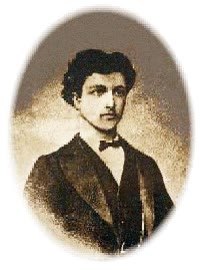
\includegraphics[width=\linewidth]{images/book3/b1-mohorovicic.jpg}

{\scriptsize 安德里亚·莫霍洛维奇。公有领域。}
\end{minipage}
\end{history}

\section{地球参考模型}

同样的推理应用于各距离上的数百万个走时，
以及地球自由振动的周期（整个行星在大地震之后会像钟一样
鸣响），便给出各深度处的速度。

\begin{definition}[地球参考模型]\label{def:b1:layered-earth:reference-model}
\emph{地球参考模型}\index{地球参考模型}是一个球对称的地球，
以地震波速 $v_P(r)$、$v_S(r)$，
密度 $\rho(r)$，以及在最完整的模型中的衰减，都仅作为
半径 $r$ 的函数给出；它须与观测到的走时、自由振动
周期、地球质量及其转动惯量相符合。应用最广的是
PREM，即初步参考地球模型（1981 年）。
\end{definition}

PREM 是依据地球的半径 \qty{6371}{km}、
质量 \qty{5.974e24}{kg} 以及\omterm{def:b1:comparative-planetology:moi}{转动惯量因子} $0.3308$ 拟合得到的。
它把地球划分为若干由不连续面隔开的区域，
其剖面（见下图）立即显示出主要的分层。

\begin{definition}[地壳、地幔、外核、内核]\label{def:b1:layered-earth:layers}
\emph{地壳}\index{地壳}是位于\omterm{def:b1:layered-earth:discontinuity}{莫霍面}之上的外层硅酸盐层。
\emph{地幔}\index{地幔}是位于\omterm{def:b1:layered-earth:discontinuity}{莫霍面}与\omterm{def:b1:layered-earth:discontinuity}{核幔边界}之间的
固态硅酸盐壳层，其深度约为 \qty{2891}{km}。
\emph{外核}\index{外核}是位于\omterm{def:b1:layered-earth:discontinuity}{核幔边界}与\omterm{def:b1:layered-earth:discontinuity}{内核边界}之间的
液态金属壳层，深度约为 \qty{5150}{km}。
\emph{内核}\index{内核}是其下方的固态金属球体，
半径约为 \qty{1220}{km}。
\end{definition}

\begin{omfigure}
\begin{tikzpicture}
\begin{axis}[omrecord, omdepth, width=0.62\linewidth, height=5.4cm, xmin=0, xmax=14, ymin=0, ymax=6371,
  xlabel={速度（\unit{km.s^{-1}}）或密度（\unit{g.cm^{-3}}）}, ylabel={深度（km）},
  ytick={0,1000,...,6000}, tick label style={font=\scriptsize}, label style={font=\small},
  clip=false, legend style={font=\scriptsize, at={(0.02,0.80)}, anchor=north west, draw=none, fill=white}]
\addplot[very thick, blue!70!black] table[x=vp, y=depth] {figdata/out/bachelor-1-prem_profiles-profiles.dat};
\addlegendentry{$v_P$}
\addplot[very thick, red!75!black] table[x=vs, y=depth] {figdata/out/bachelor-1-prem_profiles-profiles.dat};
\addlegendentry{$v_S$}
\addplot[very thick, black!70, densely dashed] table[x=rho, y=depth] {figdata/out/bachelor-1-prem_profiles-profiles.dat};
\addlegendentry{$\rho$}
\draw[black!35] (axis cs:0,670) -- (axis cs:14,670) node[right, font=\scriptsize, black] {670 km};
\draw[black!35] (axis cs:0,2891) -- (axis cs:14,2891) node[right, font=\scriptsize, black] {核幔边界};
\draw[black!35] (axis cs:0,5149.5) -- (axis cs:14,5149.5) node[right, font=\scriptsize, black] {内核边界};
\node[font=\scriptsize, anchor=west] at (axis cs:14,1700) {地幔};
\node[font=\scriptsize, anchor=west] at (axis cs:14,4000) {外核（液态）};
\node[font=\scriptsize, anchor=west] at (axis cs:14,5800) {内核（固态）};
\end{axis}
\end{tikzpicture}

\par\smallskip{\small PREM：P 波与 S 波的速度以及密度随深度的变化。
S 波速度在液态\omterm{def:b1:layered-earth:layers}{外核}中降为零，并在
固态\omterm{def:b1:layered-earth:layers}{内核}中以较小的数值重新出现；在\omterm{def:b1:layered-earth:discontinuity}{核幔边界}处，密度几乎翻倍，
而 $v_P$ 由 13.7 降至 \qty{8.1}{km.s^{-1}}；
在 \qty{400}{km} 与 \qty{670}{km} 附近的跳跃界定了过渡带。}
\end{omfigure}

\begin{table}[htbp]
\centering
\footnotesize
\setlength{\tabcolsep}{3pt}
\begin{tabular}{>{\raggedright\arraybackslash}p{0.2\linewidth}rr>{\raggedright\arraybackslash}p{0.47\linewidth}}
\hline
边界（PREM 中） & 深度（km） & 半径（km） & 变化内容 \\
\hline
\omterm{def:b1:layered-earth:discontinuity}{莫霍面} & 24.4 & 6346.6 & 上方为\omterm{def:b1:layered-earth:layers}{地壳}，下方为橄榄岩；$v_P$ 由 6.8 变为 8.1 \\
220 km 不连续面 & 220 & 6151 & PREM 中\omterm{def:b1:layered-earth:lithosphere}{低速带}的底部 \\
400 km 不连续面 & 400 & 5971 & \omterm{def:b1:rock-forming-minerals:groups}{橄榄石}转变为瓦兹利石（多数研究中为 \qty{410}{km}） \\
670 km 不连续面 & 670 & 5701 & 林伍德石转变为布里奇曼石和铁方镁石（多数研究中为 \qty{660}{km}） \\
\omterm{def:b1:layered-earth:discontinuity}{核幔边界} & 2891 & 3480 & 硅酸盐转变为液态铁；$v_S$ 由 7.3 变为 0；$\rho$ 由 5.57 变为 9.90 \\
\omterm{def:b1:layered-earth:discontinuity}{内核边界} & 5149.5 & 1221.5 & 液态铁转变为固态铁；$v_S$ 由 0 变为 3.5；$\rho$ 由 12.17 变为 12.76 \\
\hline
\end{tabular}
\caption{PREM 的主要不连续面（速度单位为 \unit{km.s^{-1}}，
密度单位为 \unit{g.cm^{-3}}）。PREM 将\omterm{def:b1:layered-earth:layers}{地壳}平均取为 \qty{24.4}{km}；实际\omterm{def:b1:layered-earth:layers}{地壳}
厚度从海洋下约 \qty{5}{km} 至
山脉下的数十千米不等。}
% ledger: usgs:crust-thickness
\label{tab:b1:layered-earth:prem}
\end{table}

这些剖面中有两个事实可以直接观测到。\omterm{def:b1:layered-earth:layers}{外核}中 $v_S$ 的消失
正是前文所述的 S 波影区：S 波只能以 P 波的形式进入地核，
而地核无法传递切变，因此它是液态的。\omterm{def:b1:layered-earth:layers}{内核}
能缓慢地传递 S 波，因此它是固态的。第二个事实来自
在本不应有 P 波的地方所观测到的微弱 P 波到达。

\begin{history}[英格·莱曼与内核]
% ledger: hjortenberg:lehmann
\begin{minipage}[t]{0.76\linewidth}\vspace{0pt}
英格·莱曼（1888--1993），任丹麦大地测量研究所
地震学部主任，研究了 1929 年新西兰布勒地震的记录，
发现 P 波到达了影区之内，
而按照理论，地核本应使其折射偏离。她在 1936 年发表了一篇题目极短的论文
\emph{P$'$}，指出若地核内含有一个较小的\omterm{def:b1:layered-earth:layers}{内核}且其 P 波速度较高，便可解释这些现象，
该\omterm{def:b1:layered-earth:layers}{内核}会将部分能量
送回地表。她的\omterm{def:b1:layered-earth:layers}{内核}如今已知是固态的，
并随地球冷却而缓慢生长。她还发现了一个
以她命名的不连续面，位于约 \qty{220}{km} 处。
\end{minipage}\hfill
\begin{minipage}[t]{0.2\linewidth}\vspace{0pt}
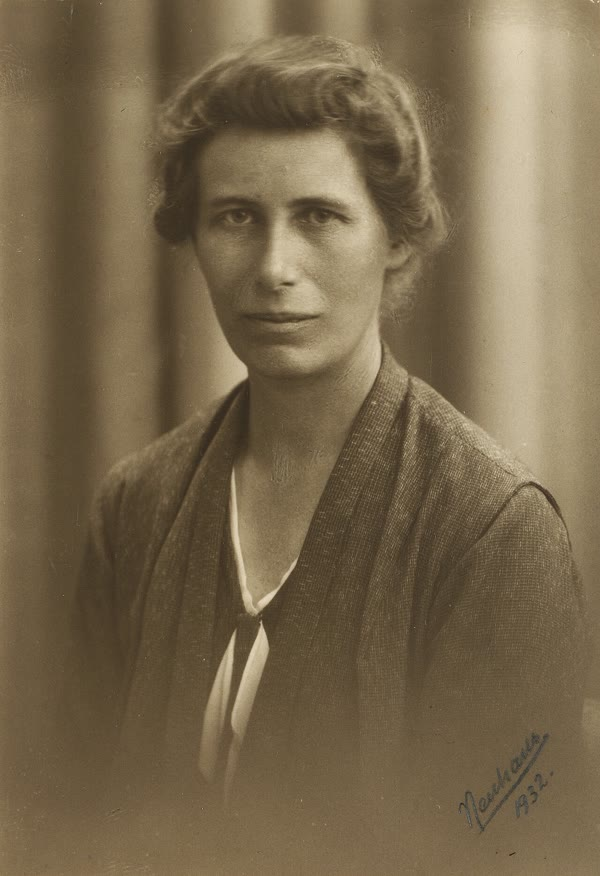
\includegraphics[width=\linewidth]{images/book3/b1-lehmann.jpg}

{\scriptsize 英格·莱曼，1932 年，Even Neuhaus 摄。公有领域。}
\end{minipage}
\end{history}

\section{由地震数据求密度、重力与压强}

地震波速只给出模量与密度的两个组合，
而非密度本身。第三个关系来自如下假设：在
成分均匀的层内，岩石仅受其上方岩石的
重量压缩。

\begin{definition}[地震参数]\label{def:b1:layered-earth:seismic-parameter}
某深度处的\emph{地震参数}\index{地震参数}为
\[
  \Phi = v_P^2 - \tfrac43 v_S^2 = \frac{K}{\rho},
\]
即体积模量除以密度，仅由两个地震波速算得
（见\cref{prop:b1:layered-earth:speeds}）。
\end{definition}

\begin{theorem}[亚当斯–威廉森方程]\label{thm:b1:layered-earth:adams-williamson}
在成分均匀、处于静力平衡且绝热压缩的区域内，
密度随半径的变化满足
\[
  \frac{\mathrm d\rho}{\mathrm dr} = -\frac{\rho(r)\,g(r)}{\Phi(r)},
\]
其中 $g(r)$ 为半径 $r$ 处的重力。
\end{theorem}

\begin{proof}
由静力平衡得 $\mathrm dP/\mathrm dr = -\rho g$（回顾一下，
此处 $\mathrm dz = -\mathrm dr$）。体积模量定义为
$K = \rho\,\mathrm dP/\mathrm d\rho$，对应所考虑的压缩过程；对于成分固定的岩石，
在无热量交换的压缩下，地震波测得的是绝热模量，
因此 $\mathrm d\rho/\mathrm dP = \rho/K$。
由链式法则，
\[
  \frac{\mathrm d\rho}{\mathrm dr} = \frac{\mathrm d\rho}{\mathrm dP}\,
  \frac{\mathrm dP}{\mathrm dr} = \frac{\rho}{K}\,(-\rho g) = -\frac{\rho g}{K/\rho}
  = -\frac{\rho g}{\Phi}. \qedhere
\]
\end{proof}

该方程在间断面处不成立，即成分或晶体结构发生变化之处，
以及温度偏离绝热线之处；但在各间断面之间，
它很好地解释了观测到的密度
随深度的增加（见下图的 (c)）。从每一区域顶部的密度出发，
向下积分，并调整起始值，直至质量和转动惯量都正确，
这便是最早密度模型的建立方法。
两个全球性数值都是密度的积分。

\begin{proposition}[质量、重力、压强与转动惯量]
\label{prop:b1:layered-earth:integrals}
对半径为 $R$、密度为 $\rho(r)$ 的球对称地球，
半径 $r$ 以内的质量、重力、压强以及
绕过球心某轴的转动惯量分别为
\[
  m(r) = \int_0^r 4\pi s^2\rho(s)\,\mathrm ds, \quad
  g(r) = \frac{G\,m(r)}{r^2}, \quad
  P(r) = \int_r^R \rho(s)\,g(s)\,\mathrm ds, \quad
  I = \frac{8\pi}{3}\int_0^R \rho(r)\,r^4\,\mathrm dr.
\]
\end{proposition}

\begin{proof}
半径为 $s$、厚度为 $\mathrm ds$ 的薄壳，其体积为
$4\pi s^2\,\mathrm ds$，由此得到第一个积分。球对称物体在某半径之外的引力
等于其内部质量集中于球心处的引力，
并且 $r$ 之外各球壳的合力为零（壳层定理，
在物理教材中不加证明地承认），由此得到 $g(r)$。
从表面（此处 $P = 0$）出发积分静力平衡方程，得到 $P(r)$。
对于转动惯量，质量为 $\mathrm dm$、半径为 $r$ 的薄球壳，
关于三根坐标轴 $x$、$y$、$z$ 的转动惯量之和为
$\int (y^2 + z^2) + (z^2 + x^2) + (x^2 + y^2)\,\mathrm dm = 2r^2\,\mathrm dm$;
由对称性，三者相等，每一个都是 $\tfrac23 r^2\,\mathrm dm$。取
$\mathrm dm = 4\pi r^2\rho\,\mathrm dr$，对各球壳求和即得 $I$。
\end{proof}

对于密度均匀的球体，$I = \tfrac{8\pi}{15}\rho R^5 = 0.4\,MR^2$。
地球的因子 $I/MR^2 = 0.3308$ 更小：其质量向中心集中，
这是支持致密地核存在的第一个论据。仅用
PREM 的密度计算，积分给出质量为 \qty{5.976e24}{kg}
（比实测的 \qty{5.972e24}{kg} 高 \qty{0.06}{\percent}），因子为 $0.3309$，
中心压强为 \qty{364}{GPa}，与 PREM 所列的表值
在 \qty{0.1}{\percent} 内一致。

\begin{omfigure}
\begin{tabular}{@{}c@{\hspace{2mm}}c@{\hspace{2mm}}c@{}}
\begin{tikzpicture}
\begin{axis}[omrecord, omdepth, width=0.35\linewidth, height=7.0cm, xmin=0, xmax=12, ymin=0, ymax=6371,
  xlabel={$g$ (\unit{m.s^{-2}})}, ylabel={深度 (km)}, ytick={0,1000,...,6000}, xtick={0,4,8,12},
  tick label style={font=\scriptsize}, label style={font=\small}]
\addplot[very thick, blue!70!black] table[x=g, y=depth] {figdata/out/bachelor-1-prem_profiles-functionals.dat};
\draw[black!35] (axis cs:0,2891) -- (axis cs:12,2891);
\draw[black!35] (axis cs:0,5149.5) -- (axis cs:12,5149.5);
\node[font=\scriptsize, anchor=south west] at (axis cs:0.3,2891) {CMB};
\node[font=\scriptsize, anchor=south west] at (axis cs:0.3,5149.5) {ICB};
\end{axis}
\end{tikzpicture}
&
\begin{tikzpicture}
\begin{axis}[omrecord, omdepth, width=0.35\linewidth, height=7.0cm, xmin=0, xmax=400, ymin=0, ymax=6371,
  xlabel={压强 $P$ (GPa)}, ytick={0,1000,...,6000}, yticklabels={}, xtick={0,200,400},
  tick label style={font=\scriptsize}, label style={font=\small}]
\addplot[very thick, red!75!black] table[x=P, y=depth] {figdata/out/bachelor-1-prem_profiles-functionals.dat};
\draw[black!35] (axis cs:0,2891) -- (axis cs:400,2891);
\draw[black!35] (axis cs:0,5149.5) -- (axis cs:400,5149.5);
\node[font=\scriptsize, anchor=south west] at (axis cs:150,2891) {\qty{136}{GPa}};
\node[font=\scriptsize, anchor=south east] at (axis cs:290,5149.5) {\qty{329}{GPa}};
\end{axis}
\end{tikzpicture}
&
\begin{tikzpicture}
\begin{axis}[omrecord, omdepth, width=0.35\linewidth, height=7.0cm, xmin=2, xmax=14, ymin=0, ymax=6371,
  xlabel={$\rho$ (\unit{g.cm^{-3}})}, ytick={0,1000,...,6000}, yticklabels={}, xtick={2,6,10,14},
  tick label style={font=\scriptsize}, label style={font=\small},
  legend style={font=\scriptsize, at={(0.97,0.97)}, anchor=north east, draw=none, fill=white}]
\addplot[very thick, black!55] table[x=rho, y=depth] {figdata/out/bachelor-1-prem_profiles-profiles.dat};
\addlegendentry{PREM}
\addplot[only marks, mark=o, mark size=1.4pt, orange!85!black, each nth point=15, unbounded coords=discard]
  table[x=rho_aw, y=depth] {figdata/out/bachelor-1-prem_profiles-adams.dat};
\addlegendentry{亚当斯–威廉森}
\end{axis}
\end{tikzpicture}
\\[2pt]
{\small (a) 重力} & {\small (b) 压强} & {\small (c) 自压缩}
\end{tabular}

\par\smallskip{\small 地球内部，数据取自 PREM。(a) 与 (b) 为重力和压强，
由 PREM 的密度，利用\cref{prop:b1:layered-earth:integrals}算得：重力
在\omterm{def:b1:layered-earth:layers}{地幔}中大体保持在 \qty{10}{m.s^{-2}} 附近，在\omterm{def:b1:layered-earth:discontinuity}{核幔边界}（CMB）处
达到峰值 \qty{10.7}{m.s^{-2}}，至地心降为零；压强在
CMB 处为 \qty{136}{GPa}，在\omterm{def:b1:layered-earth:discontinuity}{内核边界}（ICB）处为 \qty{329}{GPa}，
在地心处为 \qty{364}{GPa}。(c) 亚当斯–威廉森方程，
以 PREM 在 \qty{771}{km} 处及\omterm{def:b1:layered-earth:layers}{外核}顶部的密度为起点，
利用 PREM 的波速与重力向下积分（圆点），其结果与 PREM 符合到
\qty{0.2}{\percent} 以内：此处密度的增加即均匀物质的压缩；
而跃变则不然。}
\end{omfigure}

\omterm{def:b1:layered-earth:layers}{地幔}中重力随深度增大，是致密地核的直接结果：
随半径减小，半径以内所剩的质量减小得
比 $r^2$ 慢。穿过\omterm{def:b1:layered-earth:layers}{地幔}时 $g$ 几乎不变，压强则
几乎随深度线性增加，每百千米约增加 \qty{4.7}{GPa}。


\section{地幔：一种岩石，几种矿物组合}

上\omterm{def:b1:layered-earth:layers}{地幔}为橄榄岩，由火山带出的碎片
以及逆冲到大陆上的\omterm{def:b1:layered-earth:layers}{地幔}片段可知：按体积计，约二分之一至五分之三为\omterm{def:b1:rock-forming-minerals:groups}{橄榄石}
（在所提出的成分中为 \qtyrange{49}{62}{\percent}），其余为\omterm{def:b1:rock-forming-minerals:groups}{辉石}和一种富铝\omterm{def:b1:rock-forming-minerals:mineral}{矿物}
（依深度而定，为\omterm{def:b1:rock-forming-minerals:groups}{斜长石}、尖晶石或\omterm{def:b1:rock-forming-minerals:groups}{石榴子石}）。
随深度增加的压强不改变这一成分，
但会迫使其原子排列为更致密的结构：
\omterm{def:b1:rock-forming-minerals:polymorph}{同质多象变体}（\cref{ch:b1:rock-forming-minerals}）
依次出现。

\begin{definition}[地幔过渡带]\label{def:b1:layered-earth:transition-zone}
称\emph{地幔过渡带}\index{地幔过渡带}为
位于约 \qty{410}{km} 与
\qty{660}{km} 深处的\omterm{def:b1:layered-earth:discontinuity}{地震波速不连续面}之间的\omterm{def:b1:layered-earth:layers}{地幔}部分，其中上\omterm{def:b1:layered-earth:layers}{地幔}的\omterm{def:b1:rock-forming-minerals:groups}{橄榄石}被其
更致密的\omterm{def:b1:rock-forming-minerals:polymorph}{同质多象变体}取代，先为瓦兹利石，后为林伍德石。其上为上\omterm{def:b1:layered-earth:layers}{地幔}，
其下为下\omterm{def:b1:layered-earth:layers}{地幔}，直至\omterm{def:b1:layered-earth:discontinuity}{核幔边界}。
\end{definition}

约在 \qty{410}{km}（\qty{14}{GPa}）处，\omterm{def:b1:rock-forming-minerals:groups}{橄榄石} \ce{(Mg,Fe)2SiO4} 转变为
同式的瓦兹利石；约在 \qty{520}{km}（\qty{17.5}{GPa}）处，瓦兹利石
转变为林伍德石；\omterm{def:b1:rock-forming-minerals:groups}{辉石}溶入富硅的\omterm{def:b1:rock-forming-minerals:groups}{石榴子石}（即
majorite），直至过渡带中部，\omterm{def:b1:rock-forming-minerals:groups}{石榴子石}
占据了全部\omterm{def:b1:rock-forming-minerals:groups}{辉石}的位置，因此该带略多于一半为\omterm{def:b1:rock-forming-minerals:groups}{橄榄石}的\omterm{def:b1:rock-forming-minerals:polymorph}{同质多象变体}，其余为
\omterm{def:b1:rock-forming-minerals:groups}{石榴子石}。约在 \qty{660}{km} 处、压强接近 \qty{24}{GPa} 时，林伍德石
分解为
两种\omterm{def:b1:rock-forming-minerals:mineral}{矿物}，以镁\omterm{def:b1:rock-forming-minerals:solid-solution}{端元}为例写作
\[
  \ce{Mg2SiO4 -> MgSiO3 + MgO}:
\]
布里奇曼石 \ce{(Mg,Fe)SiO3}，具钙钛矿结构，以及
铁方镁石 \ce{(Mg,Fe)O}。下\omterm{def:b1:layered-earth:layers}{地幔}与上\omterm{def:b1:layered-earth:layers}{地幔}成分相同，其体积组成约为
布里奇曼石约 \qty{75}{\percent}、铁方镁石 \qty{17}{\percent}，
以及 \qty{8}{\percent} 的钙硅酸盐钙钛矿（按体积计），
其密度与速度符合\omterm{def:b1:layered-earth:reference-model}{参考地球模型}。因此布里奇曼石
是地球上含量最多的\omterm{def:b1:rock-forming-minerals:mineral}{矿物}；它直至 2014 年才被命名，
在此之前，天然颗粒已在一块受过强烈冲击的陨石中被描述。
% ledger: frost:mantle-transitions, sun:lower-mantle, tschauner:bridgmanite

每次转变都生成更致密的\omterm{def:b1:rock-forming-minerals:mineral}{矿物}，因而同时提高密度，
并提高地震波速：这些转变正是剖面中的不连续面
（见下图）。它们的深度
并不固定。相变发生的压强取决于
温度，而这种依赖关系的斜率（即克拉珀龙斜率，将在下一册大学分册中讨论）
使 \qty{410}{km} 处的不连续面上移，并使下沉板片冷岩石中的
\qty{660}{km} 处的不连续面下移。测绘不连续面的起伏形态，
是确定\omterm{def:b1:layered-earth:layers}{地幔}中冷区与热区的一种方法。

\begin{omfigure}
\begin{tikzpicture}[x=0.075mm, y=-0.062mm, font=\scriptsize]
% schematic volume fractions (ledger frost:mantle-transitions, sun:lower-mantle)
\def\W{1000}
% upper mantle 0-410: olivine 60, pyroxenes 30, garnet 10
\fill[green!45!olive!60] (0,0) rectangle (600,410);
\fill[brown!35] (600,0) rectangle (900,410);
\fill[red!35] (900,0) rectangle (1000,410);
% 410-520 wadsleyite 60, garnet 40 ; 520-660 ringwoodite 60, garnet 40
\fill[teal!50] (0,410) rectangle (600,520);
\fill[blue!35] (0,520) rectangle (600,660);
\fill[red!45] (600,410) rectangle (1000,660);
% 660-1000 bridgmanite 75, ferropericlase 17, Ca-perovskite 8
\fill[orange!45] (0,660) rectangle (750,1000);
\fill[gray!40] (750,660) rectangle (920,1000);
\fill[yellow!50] (920,660) rectangle (1000,1000);
\draw (0,0) rectangle (1000,1000);
\foreach \d in {410,520,660} \draw[thick] (0,\d) -- (1000,\d);
\node at (300,205) {橄榄石};
\node[align=center] at (750,205) {辉石};
\node[rotate=90] at (950,205) {石榴子石};
\node at (300,465) {瓦兹利石};
\node at (300,590) {林伍德石};
\node[align=center] at (800,590) {石榴子石};
\node at (375,830) {布里奇曼石};
\node[rotate=90, align=center] at (835,830) {铁方镁石};
\node[rotate=90] at (960,830) {Ca-钙钛矿};
\foreach \d in {0,200,410,520,660,800,1000} \node[anchor=east] at (-10,\d) {\d};
\node[rotate=90, anchor=south] at (-160,500) {深度（km）};
\foreach \p in {0,25,50,75,100} \node[anchor=north] at (\p*10,1010) {\p};
\node[anchor=north] at (500,1080) {体积百分比};
\node[anchor=west, align=left] at (1030,205) {上地幔};
\node[anchor=west, align=left] at (1030,535) {过渡 \\带};
\node[anchor=west, align=left] at (1030,830) {下地幔};
\end{tikzpicture}

\par\smallskip{\small 随深度变化的橄榄岩\omterm{def:b1:layered-earth:layers}{地幔}\omterm{def:b1:rock-forming-minerals:mineral}{矿物}，以体积分数表示
（示意图：边界画成清晰的线，分数取正文所给范围内的整数值）。
成分不随深度改变；\omterm{def:b1:rock-forming-minerals:mineral}{矿物}则在约 410、520 与
\qty{660}{km} 处发生改变。}
\end{omfigure}

\omterm{def:b1:layered-earth:layers}{地幔}底部的 D$''$ 层（D 双撇，一个源自早期地球模型的名称），
其速度梯度不同于下\omterm{def:b1:layered-earth:layers}{地幔}的其余部分；PREM 将其取为\omterm{def:b1:layered-earth:layers}{地幔}最底部的
\qty{150}{km}。该层在地震上是非均匀的：
存在速度极低的斑块、陡峭的梯度与反射体。它被认为是炽热地核与
\omterm{def:b1:layered-earth:layers}{地幔}之间的边界层，
或许也是旧板片的“墓场”。
% ledger: prem:dpp

\section{地核}

地核主要由铁组成。其密度、速度与产生磁场的能力都指向金属，
而在陨石与太阳所显示的常见元素中，铁是密度足够大的元素里
最丰富的一种。镍在铁陨石中含量丰富，与铁相伴。
但地核
并非纯粹的铁镍合金。
\begin{itemize}
  \item 地核的密度比同一压强与温度下的纯铁低
        \qtyrange{5}{10}{\percent}，因而必须含有轻元素，
        其中硅、硫、碳、氧与氢是
        可能的候选者。
  \item 在\omterm{def:b1:layered-earth:discontinuity}{内核边界}处，密度跃变约为 \qty{4.5}{\percent}，
        这一幅度对于单一金属的凝固而言过大：\omterm{def:b1:layered-earth:layers}{内核}同样含有轻元素，
        但含量较少，为百分之几，
        而液态\omterm{def:b1:layered-earth:layers}{外核}中为 \qtyrange{5}{10}{\percent}。
\end{itemize}
% ledger: badro:core
这一差异带来一个后果。地球冷却时——目前其\omterm{def:b1:layered-earth:layers}{地幔}每十亿年约降温
\qty{100}{\degreeCelsius}——地核的液体
在\omterm{def:b1:layered-earth:layers}{内核}上凝固，使\omterm{def:b1:layered-earth:layers}{内核}不断长大，并且
% ledger: bellini:cooling
凝固使大部分轻元素留在液体中。被释放于\omterm{def:b1:layered-earth:layers}{外核}底部的轻质液体上升，
这种浮力被认为有助于搅动\omterm{def:b1:layered-earth:layers}{外核}，
并驱动使地球获得磁场的
发电机。

\section{力学分层：岩石圈与软流圈}

上述各层依据成分和相态划分：\omterm{def:b1:layered-earth:layers}{地壳}与\omterm{def:b1:layered-earth:layers}{地幔}是
不同的岩石，\omterm{def:b1:layered-earth:layers}{外核}与\omterm{def:b1:layered-earth:layers}{内核}是不同的状态。板块构造需要的是
另一种按强度进行的划分，它与前一种相互交叉。

\begin{definition}[岩石圈、软流圈、低速带]
\label{def:b1:layered-earth:lithosphere}
称\emph{岩石圈}\index{岩石圈}为地球刚性的外壳，
即\omterm{def:b1:layered-earth:layers}{地壳}和最上部的\omterm{def:b1:layered-earth:layers}{地幔}，在地质时间尺度上表现为一个强层，
并被划分为若干板块。
\emph{软流圈}\index{软流圈}是其下方上\omterm{def:b1:layered-earth:layers}{地幔}中较弱的一层，
在缓慢流动中发生形变，使板块得以运动。
\emph{低速带}\index{低速带}是岩石圈之下的深度范围，
在该范围内地震波速，尤其是 S 波速，
明显低于其紧邻的上方和下方。
\end{definition}

\omterm{def:b1:layered-earth:lithosphere}{岩石圈}并非一种岩石，而是一个温度范围：\omterm{def:b1:layered-earth:layers}{地幔}橄榄岩
在低温时坚固，高温时缓慢蠕变，其底界大致是一个
等温面。它在洋中脊下方很薄，那里热\omterm{def:b1:layered-earth:layers}{地幔}上升，
在最古老的洋底之下厚约 \qty{140}{km}，在大陆之下厚 \qtyrange{40}{280}{km}，
最厚处位于古老克拉通之下；\omterm{def:b1:layered-earth:lithosphere}{软流圈}顶部约位于
\qtyrange{80}{200}{km} 深处。从地震学看，\omterm{def:b1:layered-earth:lithosphere}{软流圈}表现为\omterm{def:b1:layered-earth:lithosphere}{低速带}，
接近其熔化条件：在 PREM 模型中，
S 波速度自\omterm{def:b1:layered-earth:discontinuity}{莫霍面}向下至 \qty{220}{km} 处略有减小，
然后又突然增大。强度如何随温度变化以及为何如此，
将在\cref{ch:b1:stress-strain-rheology}中讨论。

\begin{inthefield}[地震台站]
\begin{minipage}[t]{0.55\linewidth}\vspace{0pt}
参考模型所依据的走时资料来自永久性台站。
宽频带地震仪可记录地面运动，其周期从百分之一秒到数小时，
它安装在直接置于裸岩上的混凝土墩上，与地下洞室地面隔离，
并罩以保温罩，使温度保持稳定：
温度哪怕只变化几分之一度、一阵穿堂风或一辆驶过的卡车，都会在记录上显现。
数据记录仪用卫星信号为每个采样标注时间，
记录数据则实时传送至公开共享数据的数据中心。
由这类台站组成的台网可定位每次大地震并为其计时；从其记录中拾取的到时
被用来反演各深度处的波速。
\end{minipage}\hfill
\begin{minipage}[t]{0.42\linewidth}\vspace{0pt}
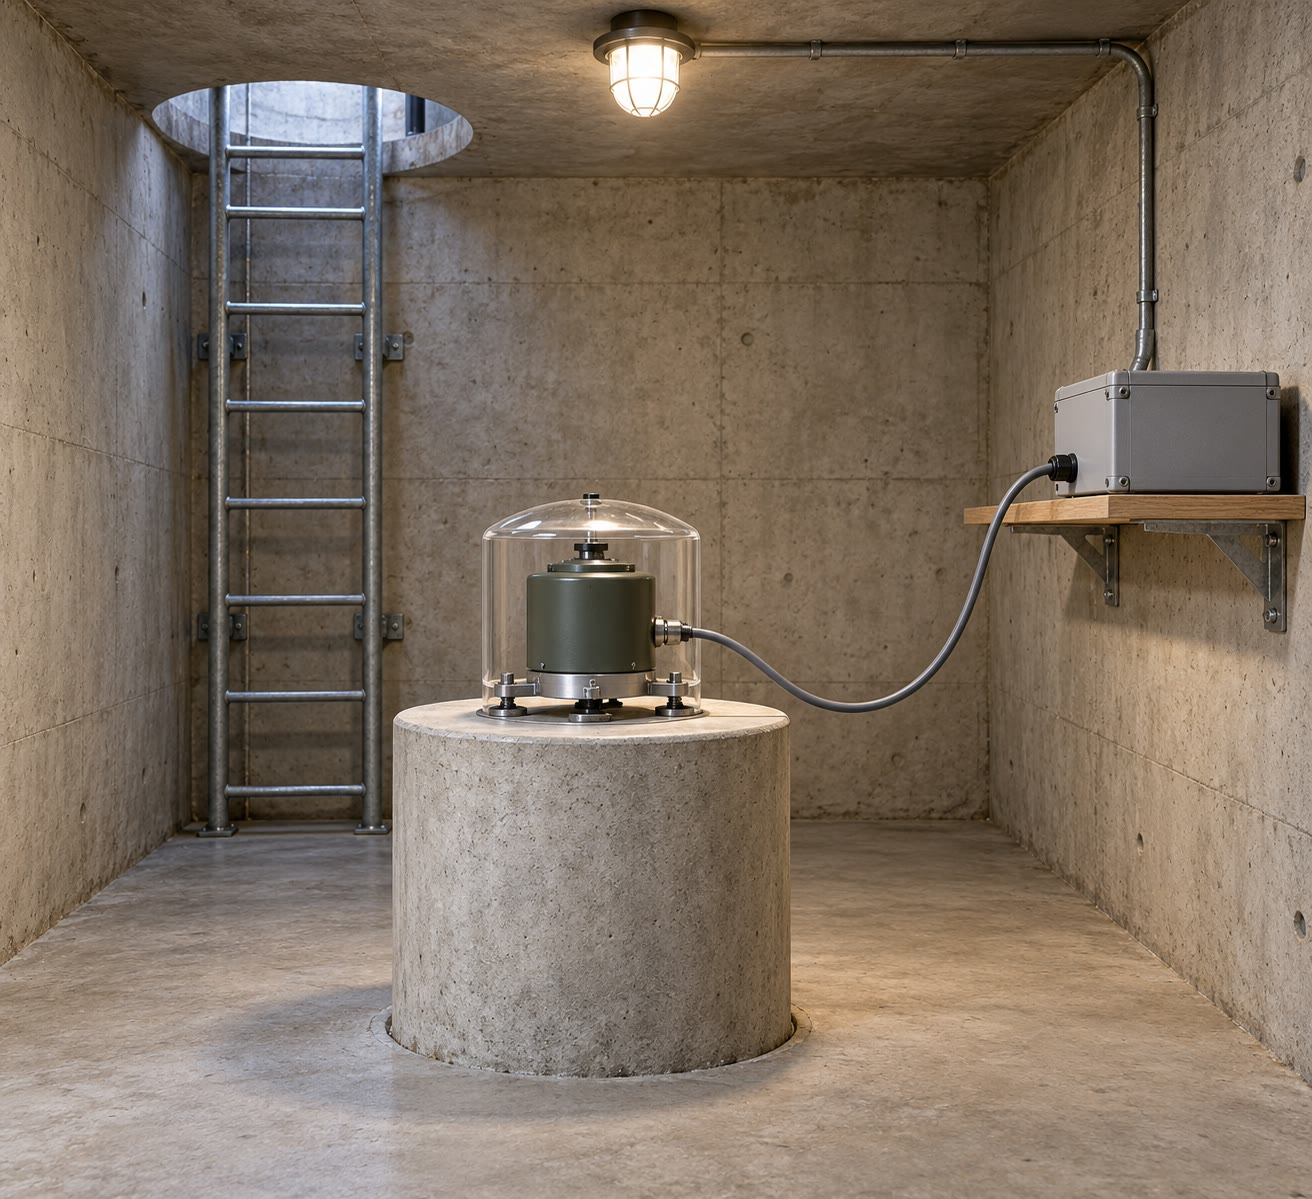
\includegraphics[width=\linewidth]{images/book3/ai/b1-seismometer-vault.jpg}

{\scriptsize 地下洞室中墩座上的宽频带地震仪，
数据记录仪装于墙上（AI 生成的示意图）。}
\end{minipage}
\end{inthefield}

\section{练习}

\begin{exercise}[$\star$]\label{exo:b1:layered-earth:1}
已知 PREM 半径 $R = \qty{6371}{km}$，$r_{\text{CMB}} = \qty{3480}{km}$ 和
$r_{\text{ICB}} = \qty{1221.5}{km}$，计算地核与\omterm{def:b1:layered-earth:layers}{内核}
分别占地球体积的比例。
% ledger: prem:cmb, prem:icb
\end{exercise}

\begin{exercise}[$\star$]\label{exo:b1:layered-earth:2}
紧邻\omterm{def:b1:layered-earth:discontinuity}{核幔边界}上方，PREM 给出 $v_P = \qty{13.7166}{km.s^{-1}}$，
$v_S = \qty{7.26466}{km.s^{-1}}$，$\rho = \qty{5.56645}{g.cm^{-3}}$；紧邻其下方，
$v_P = \qty{8.06482}{km.s^{-1}}$，$v_S = 0$，$\rho = \qty{9.90349}{g.cm^{-3}}$。
计算两侧的\omterm{def:b1:layered-earth:seismic-parameter}{地震参数}和体积模量（以 GPa 为单位）。
跨越该边界时，哪一个量变化最大？
% ledger: data:prem, prem:cmb
\end{exercise}

\begin{exercise}[$\star$]\label{exo:b1:layered-earth:3}
一层厚 \qty{30}{km}、波速为 \qty{6.2}{km.s^{-1}} 的\omterm{def:b1:layered-earth:layers}{地壳}，覆于
波速为 \qty{8.1}{km.s^{-1}} 的\omterm{def:b1:layered-earth:layers}{地幔}之上。计算临界角、临界距离和
\omterm{def:b1:layered-earth:head-wave}{交叉距离}。
\end{exercise}

\begin{exercise}[$\star$]\label{exo:b1:layered-earth:4}
地核的质量为 \qty{1.94e24}{kg}，半径为 \qty{3480}{km}。计算
\omterm{def:b1:layered-earth:discontinuity}{核幔边界}处的重力，并将其与地表重力
\qty{9.82}{m.s^{-2}} 相比较。为何它更大？
\end{exercise}

\begin{exercise}[$\star\star$]\label{exo:b1:layered-earth:5}
在折射剖面上，\omterm{def:b1:layered-earth:head-wave}{首波}到时分别为 \qty{10.0}{s}（位于
\qty{60}{km} 处）、\qty{33.3}{s}（位于 \qty{200}{km} 处）和 \qty{45.8}{s}（位于
\qty{300}{km} 处）；过第一点的直线经过原点。
求 $v_1$、$v_2$、截距时间和界面深度，并
用\omterm{def:b1:layered-earth:head-wave}{交叉距离}检验结果。
\end{exercise}

\begin{exercise}[$\star\star$]\label{exo:b1:layered-earth:6}
证明均匀球体满足 $I = 0.4\,MR^2$。随后计算质量以及
两层地球的\omterm{def:b1:comparative-planetology:moi}{转动惯量因子} $I/MR^2$：半径为 \qty{3480}{km} 的地核，
密度为 \qty{11.0}{g.cm^{-3}}，位于密度为 \qty{4.45}{g.cm^{-3}} 的\omterm{def:b1:layered-earth:layers}{地幔}之中，
其中 $R = \qty{6371}{km}$。与 \num{5.972e24} 千克和 $0.3308$ 比较。
\end{exercise}

\begin{exercise}[$\star\star$]\label{exo:b1:layered-earth:7}
在 \qty{1471}{km} 深处，PREM 给出 $v_P = \qty{12.16}{km.s^{-1}}$，
$v_S = \qty{6.673}{km.s^{-1}}$，$\rho = \qty{4.86}{g.cm^{-3}}$，重力加速度为
\qty{9.9}{m.s^{-2}}。计算由
亚当斯–威廉森方程给出的密度梯度（单位为 \unit{g.cm^{-3}} 每 \qty{1000}{km}），并与
PREM 的密度进行比较：在 \qty{1471}{km} 处为 \num{4.844}，在
\qty{2471}{km} 处为 \num{5.357}。
% ledger: data:prem
\end{exercise}

\begin{exercise}[$\star\star$]\label{exo:b1:layered-earth:8}
估算 \qty{670}{km} 深处的压强，所用平均密度为
\qty{3.57}{g.cm^{-3}}，重力加速度为 \qty{9.9}{m.s^{-2}}。该深度处预期发生
哪一种\omterm{def:b1:rock-forming-minerals:mineral}{矿物}相变？
% ledger: frost:mantle-transitions
\end{exercise}

\begin{exercise}[$\star\star$]\label{exo:b1:layered-earth:9}
地核的平均密度为 \qty{10.90}{g.cm^{-3}}；在\omterm{def:b1:layered-earth:discontinuity}{内核边界}处，
其密度上方为 \qty{12.166}{g.cm^{-3}}，下方为 \qty{12.764}{g.cm^{-3}}。
(a)~若相同条件下的铁比\omterm{def:b1:layered-earth:layers}{外核}密度大 \qtyrange{5}{10}{\percent}，
则该处液态铁的密度范围是多少？
(b)~计算\omterm{def:b1:layered-earth:discontinuity}{内核边界}处的密度跃变（以百分比表示），
并与近期研究的 \qty{4.5}{\percent} 进行比较。
(c)~若跃变大于仅由凝固所能产生的跃变，
这对轻元素说明了什么？
% ledger: badro:core, prem:icb
\end{exercise}

\begin{exercise}[$\star\star\star$]\label{exo:b1:layered-earth:10}
证明反射波走时 $t_r(x) = \sqrt{x^2 + 4h^2}/v_1$ 与
\cref{thm:b1:layered-earth:two-layer} 中的\omterm{def:b1:layered-earth:head-wave}{首波}走时
在 $x = 2h\tan i_c$ 处相等且斜率相同，并证明在此之后 $t_r > t_{\text{首波}}$。
请加以解释。
\end{exercise}

\begin{exercise}[$\star\star\star$]\label{exo:b1:layered-earth:11}
对于密度均匀为 $\rho$ 的地球，证明 $g(r) = \tfrac43\pi G\rho r$
且 $P(r) = \tfrac23\pi G\rho^2(R^2 - r^2)$。取
$\rho = \qty{5513}{kg.m^{-3}}$，$R = \qty{6371}{km}$，计算中心压强，并与 PREM 的
\qty{363.85}{GPa} 进行比较。
% ledger: earth:density, prem:centre
\end{exercise}

\begin{exercise}[$\star\star\star$]\label{exo:b1:layered-earth:12}
证明若 $g/\Phi$ 在某一层内为常数，则由亚当斯–威廉森方程可得
$\rho = \rho_0\exp\bigl(g(z - z_0)/\Phi\bigr)$，其中 $z$ 为深度。
将其应用于\omterm{def:b1:layered-earth:layers}{外核}，从 \qty{2891}{km}（$\rho_0 =
\qty{9.90}{g.cm^{-3}}$）到 \qty{5149.5}{km}，取平均值
$g = \qty{7.9}{m.s^{-2}}$，$\Phi = \qty{87}{km^2.s^{-2}}$；并与
PREM 在\omterm{def:b1:layered-earth:discontinuity}{内核边界}处的 \qty{12.17}{g.cm^{-3}} 进行比较。
% ledger: prem:icb
\end{exercise}

\section{问题：称量地球的各壳层}

\begin{problem}[{周末问题——由 PREM 构造的四壳层地球的体积、质量与
转动惯量，与实测质量和转动惯量比较；
地球深部的重力与压强}]
\label{pb:b1:layered-earth:1}
% values: calc/ch09.py; mean densities rounded from figdata prem_profiles (values part)
% ledger: data:prem, prem:constraints, prem:centre, prem:cmb, earth:mass, earth:MoI, const:G
地球按 PREM 的半径切分为四个壳层，每个壳层取其在 PREM 中的
平均密度（已取整）：
\begin{center}
\small
\begin{tabular}{lccc}
\hline
壳层 & 起始 (km) & 终止 (km) & 平均密度 (\unit{g.cm^{-3}}) \\
\hline
\omterm{def:b1:layered-earth:layers}{地壳}、上\omterm{def:b1:layered-earth:layers}{地幔}与过渡带 & 5701 & 6371 & 3.57 \\
下\omterm{def:b1:layered-earth:layers}{地幔} & 3480 & 5701 & 4.90 \\
\omterm{def:b1:layered-earth:layers}{外核} & 1221.5 & 3480 & 10.90 \\
\omterm{def:b1:layered-earth:layers}{内核} & 0 & 1221.5 & 12.89 \\
\hline
\end{tabular}
\end{center}
取 $G = \qty{6.674e-11}{m^3.kg^{-1}.s^{-2}}$。地球的实测质量为
\qty{5.972e24}{kg}，其\omterm{def:b1:comparative-planetology:moi}{转动惯量因子} $I/MR^2 = 0.3308$。

\medskip
\noindent\textbf{第一部分——体积。}
\begin{enumerate}
  \item 计算地球的体积。
  \item 计算各壳层的体积。
  \item 各壳层各占总体积的比例是多少？哪一壳层
        最大？
  \item 地核占总体积的比例是多少？
\end{enumerate}

\noindent\textbf{第二部分——质量。}
\begin{enumerate}[resume]
  \item 计算各壳层的质量。
  \item 将它们相加，并将总质量与实测质量进行比较。
  \item 推算模型地球的平均密度。
  \item \omterm{def:b1:layered-earth:layers}{内核}的质量占总质量的比例是多少？
  \item \omterm{def:b1:layered-earth:layers}{地幔}与\omterm{def:b1:layered-earth:layers}{地壳}合在一起的质量占总质量的比例是多少？
  \item 比较地核在体积和质量中所占的份额，并加以解释。
\end{enumerate}

\noindent\textbf{第三部分——转动惯量。}
\begin{enumerate}[resume]
  \item 由\cref{prop:b1:layered-earth:integrals}可证明，介于
        $r_1$ 与 $r_2$ 之间的均匀壳层的转动惯量为 $I = \tfrac{8\pi}{15}\rho\,(r_2^5 - r_1^5)$。
  \item 计算各壳层的转动惯量。
  \item 哪一壳层的贡献最大？为何\omterm{def:b1:layered-earth:layers}{内核}的贡献
        几乎为零？
  \item 将它们相加，并计算模型的 $I/MR^2$。
  \item 将其与 $0.3308$ 以及均匀球体的 $0.4$ 进行比较。
  \item 在每个真实壳层内部，密度随深度增加。这能否
        解释模型因子偏大的原因？请加以说明。
\end{enumerate}

\noindent\textbf{第四部分——重力与压强。}
\begin{enumerate}[resume]
  \item 计算模型表面的重力加速度。
  \item 计算\omterm{def:b1:layered-earth:discontinuity}{核幔边界}处的重力加速度。
  \item 计算\omterm{def:b1:layered-earth:layers}{地幔}与\omterm{def:b1:layered-earth:layers}{地壳}合在一起的平均密度。
  \item \omterm{def:b1:layered-earth:layers}{地幔}中的重力加速度接近 \qty{10}{m.s^{-2}}。估算
        \omterm{def:b1:layered-earth:discontinuity}{核幔边界}处的压强，并与 PREM 的
        \qty{135.75}{GPa} 进行比较。
  \item 计算地核的平均密度，以及在均匀地核中从\omterm{def:b1:layered-earth:discontinuity}{核幔边界}到地心的
        压强增量，
        $\tfrac23\pi G\rho_c^2 r_c^2$（将\cref{exo:b1:layered-earth:11}仅应用于地核）。
  \item 将两者相加，估算地心压强，并与 PREM 的
        \qty{363.85}{GPa} 进行比较。为何估算值偏低？
  \item 模型中哪些数值可用实测值检验，
        哪些只能与 PREM 本身比较？
  \item 地核的质量占地球总质量的比例是多少？
\end{enumerate}
\end{problem}
